\documentclass[11pt,a4paper]{article}
\usepackage[top=1.00in, bottom=1.0in, left=1.1in, right=1.1in]{geometry}
\usepackage{graphicx}
\usepackage[numbers]{natbib}
\bibliographystyle{..//bib/styles/nature.bst}

\usepackage[export]{adjustbox}

\usepackage{Sweave}
\begin{document}
\Sconcordance{concordance:microletter_agformet.tex:microletter_agformet.Rnw:%
1 44 1 50 0}


\vspace{1.5ex}

\pagenumbering{gobble}

\noindent{Dear Dr. Novick??? I'm not sure... :}
\vspace{3ex}\\
\noindent Please consider our manuscript entitled `Variation across space, species and methods in models of spring phenology' as a Research Paper for \textit{Agricultural and Forest Meteorology}. \\

As climate change and urbanization shift increase, predicting spring plant phenology in temperate forests is critical for forecasting important processes such as carbon storage. The growing degree day (GDD) model is a major forecasting method but required GDD is predicted to shift with changes in climate, especially warmer winters. In this study, we combine simulations, observations from one urban arboretum and one rural forested site, and Bayesian hierarchical models to assess how consistent GDD models of budburst are across species and landscapes. We also compare two methods to measure climate data (i.e., weather station data and hobo logger data). In addition to disentangling myriad information from observations, simulations and Bayesian models, we also develop an interactive Shiny application that aims to enhance understanding and implementation of results into future studies. \\

We find that estimated GDD thresholds can vary up to 20\% across sites and methods. Our results suggest that forecasts based on GDD models for spring phenology have inherent accuracy issues, and vary strongly across space, species and warming. Our research improves our improved understanding of GDD models, and alongside efforts to build more mechanistic models, we can refine our understanding of spring phenology and, in turn, improve forecasts for temperate forests. \\

All authors substantially contributed to this work and approved of this version for submission. The manuscript is 4680 words, with a 278 word summary and five figures. We hope that you will find it suitable for publication in \textit{Agricultural and Forest Meteorology}. Thank you for your consideration. \\

\vspace{1.5ex}
\noindent Sincerely, \\
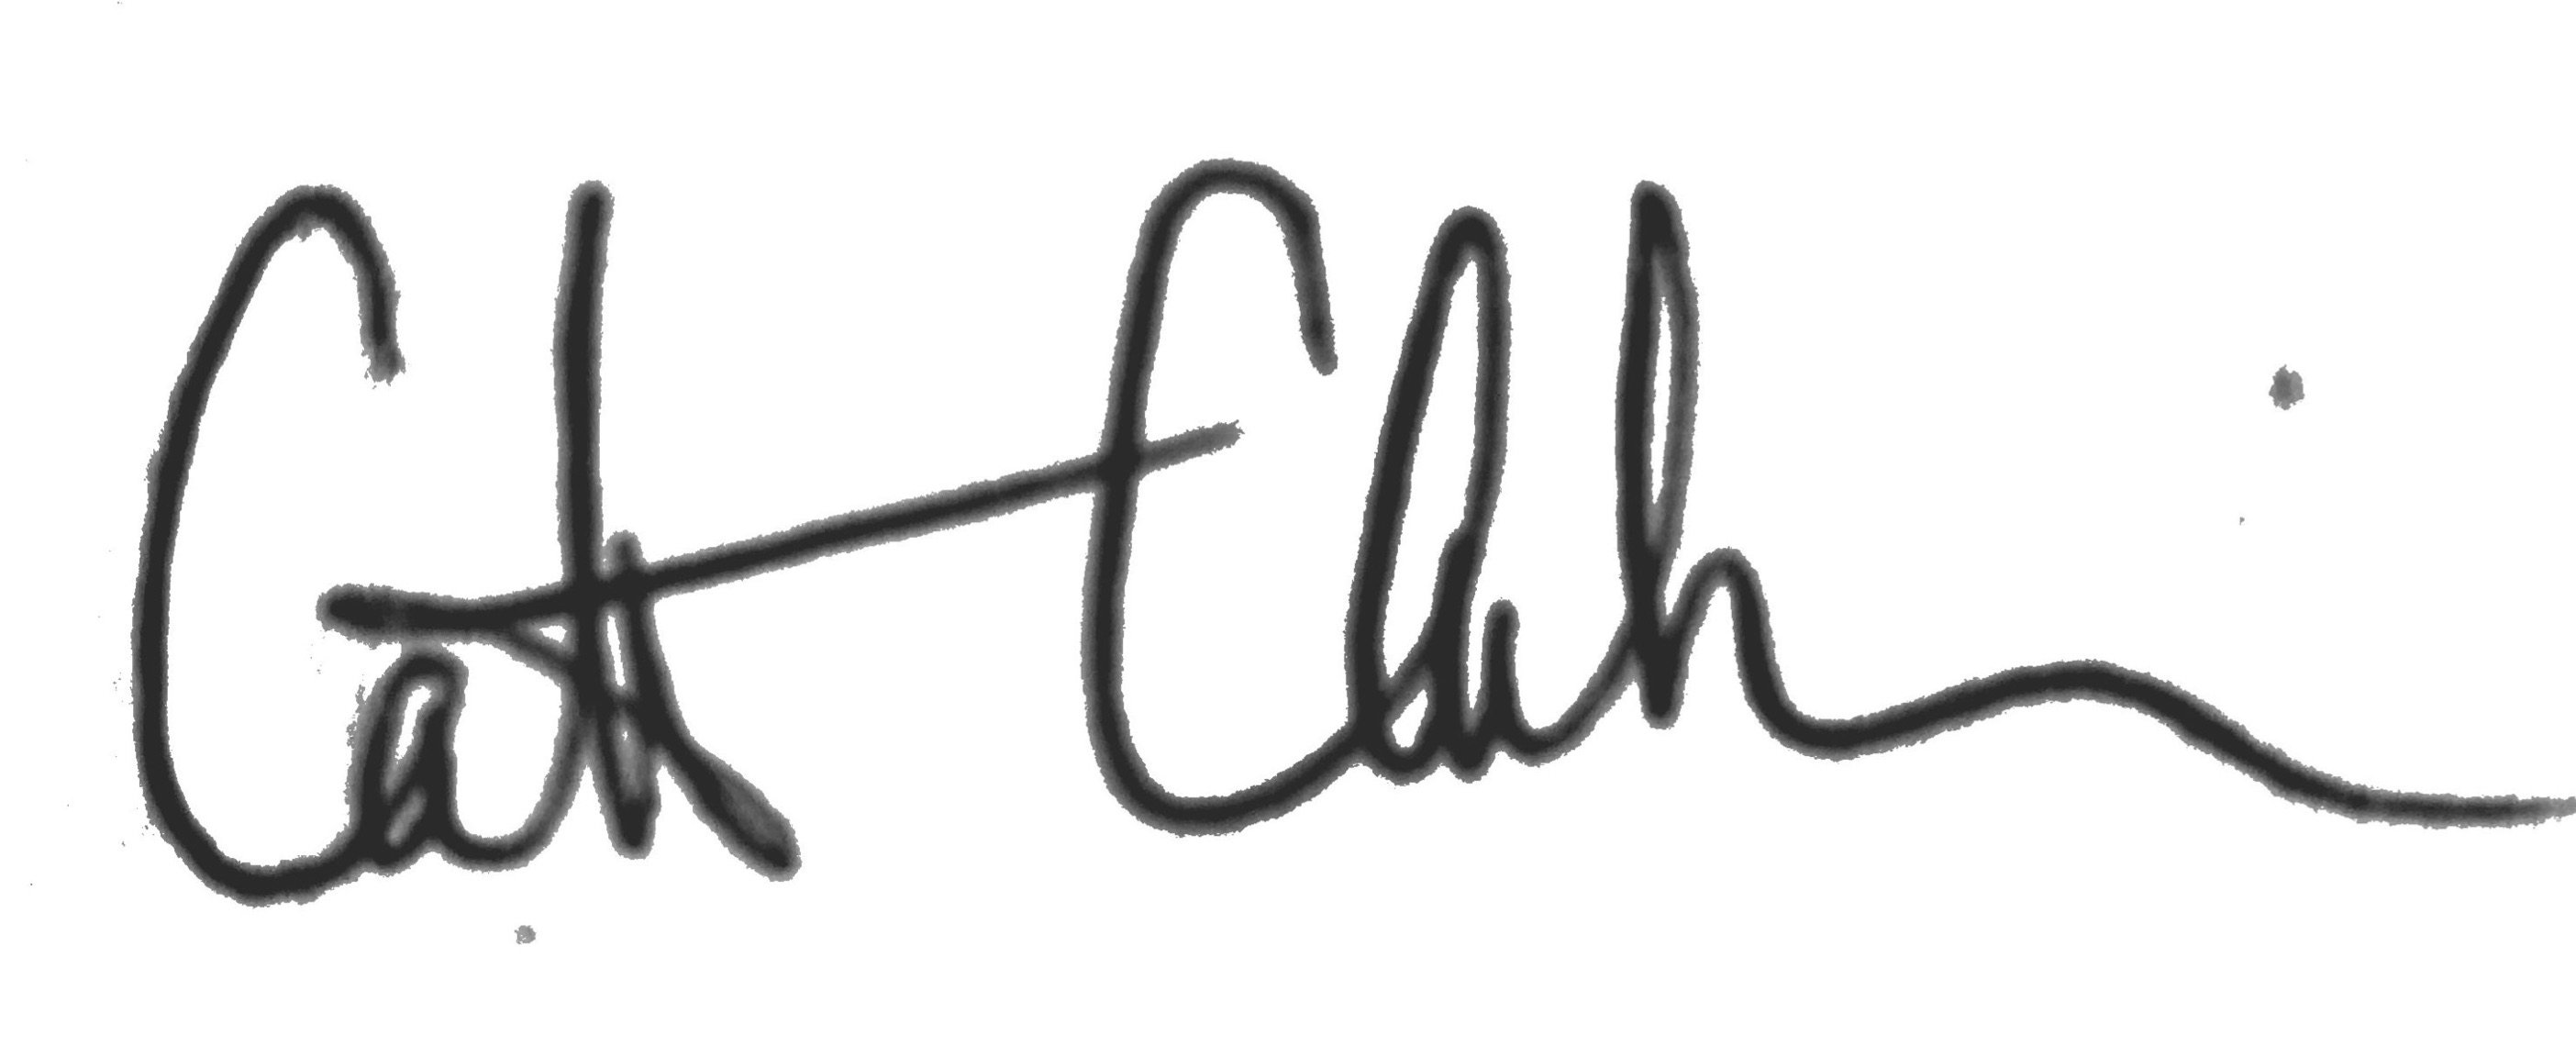
\includegraphics[width=0.2\textwidth]{full_signature.jpg} \\
\noindent Catherine Chamberlain (on behalf of my co-authors)
\vspace{2ex}\\
\noindent Authors:\\
C. J. Chamberlain $^{1,2,3}$ \& E. M. Wolkovich $^{1,2,4}$
\vspace{2ex}\\
\emph{Author affiliations:}\\
$^{1}$Arnold Arboretum of Harvard University, 1300 Centre Street, Boston, Massachusetts, USA; \\
$^{2}$Organismic \& Evolutionary Biology, Harvard University, 26 Oxford Street, Cambridge, Massachusetts, USA; \\
$^{3}$Conservation International, Arlington, VA, USA;\\
$^{4}$Forest \& Conservation Sciences, Faculty of Forestry, University of British Columbia, 2424 Main Mall, Vancouver, BC V6T 1Z4;\\
\vspace{2ex}
$^*$Corresponding author: 248.953.0189; cchamberlain@conservation.org\\


\end{document}
